The Microsoft Kinect utilizes an infrared emitter and a IR monochrome CMOS (complimentary metal-oxide semiconductor) sensor to measure and sense depth ~\cite{MicrosoftCorporation1:2013:Online, MicrosoftCorporation2:2013:Online}.  The emitter emits the infrared light beams and the CMOS sensor reads these IR beams that are reflected back to the sensor.  These beams are then converted into depth information measuring the distance between an object and the sensor.  Due to this functionality, we were able to measure and track depth and obtain an x, y, and z point for each of the data points.   During the entirety of the workout, the participant stood facing the Kinect sensor in order to accurately measure their movements.  The interface we designed to track the workout movement featured the skeleton drawing of the participant as well as a "Start" button to indicate that the participant session has begun, a button for each of the seven moves, and a "Stop" button to stop tracking the participant while they are completing the resting move.  Please see figure 2 for a screen capture of the Kinect interface we designed.  \\
\begin{figure} [h]
	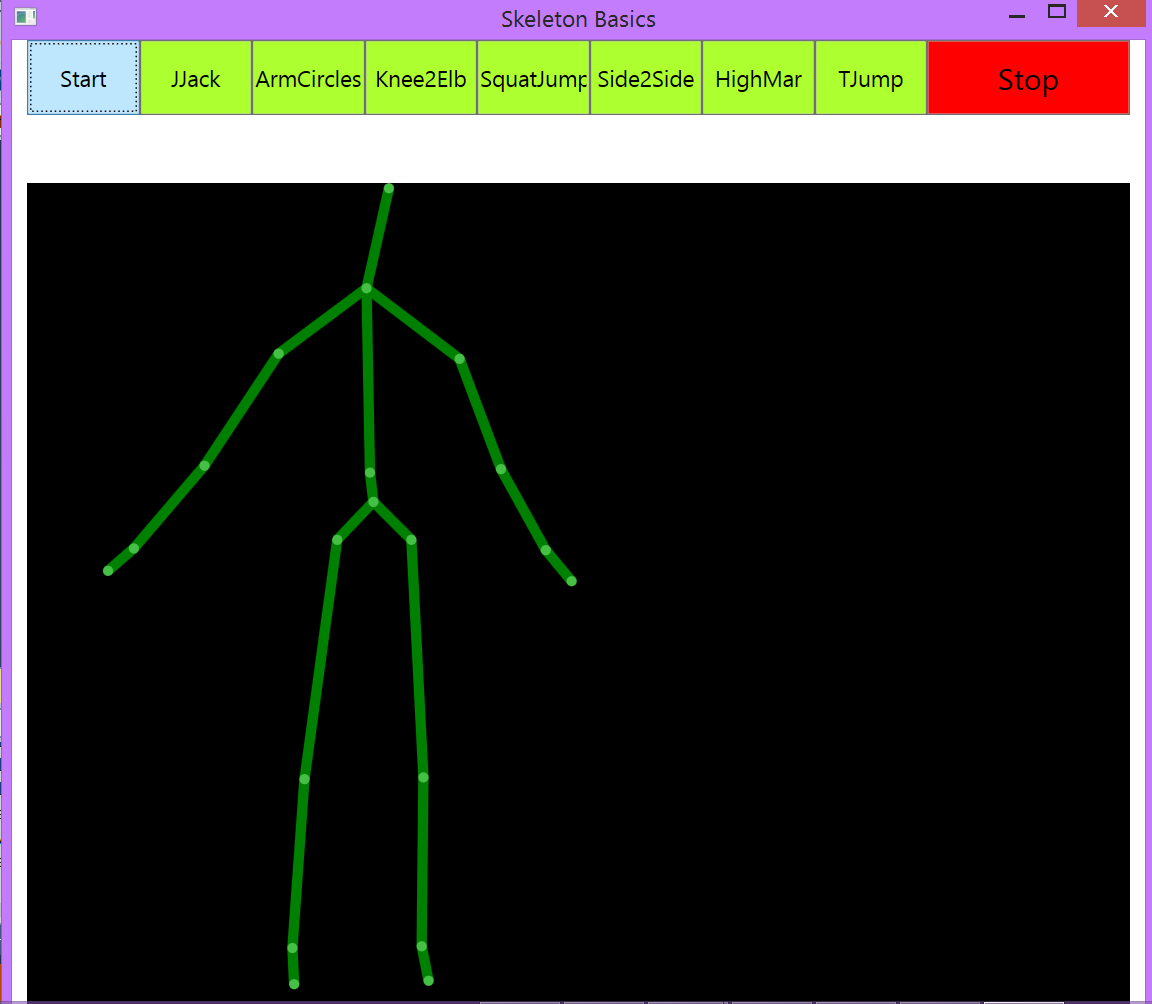
\includegraphics[width=0.5\textwidth]{images/figure2}
\caption{The Kinect Sensor Interface}
\end{figure}
Regarding the technical specificiation of the Kinect and its capabilities, the SDK features built in functionality that provides a deep understanding of human characteristics.  The SDK features skeletal tracking, facial tracking, and gesture recognition.  The Kinect Fusion algorithm makes it relatively computationally inexpensive to continuously scan the scene by recovering the camera position from the previously scanned point.  We took advantage of both the skeletal tracking functionality and the Kinect Fusion algorithm to store the x, y, and z points of the left ankle, right ankle, left elbow, right elbow, left foot, right foot, head, left wrist, right wrist, and spine.  From this we were able to use our post processing script to determine the number of exercises moves done within the time period and, for a sample of the exercise moves (High marches, squat jumps, and jumping jacks), the participants' from while completing that move.